\chapter{Convenciones \index{Convenciones} adoptadas para \textsc{XLogo}}
   \label{Convenciones-XLogo}

Esta secci\'on define aspectos claves acerca del lenguaje \textsc{Logo}
en general, y sobre \textsc{XLogo} en particular.

\section{Comandos \index{Comandos} y su interpretaci\'on}
   \label{Comandos}

El lenguaje \textsc{Logo} permite que ciertos eventos sean iniciados
por comandos internos. Estos comandos son llamados
\textit{primitivas}. \index{Primitivas}Cada primitiva puede tener un
cierto n\'umero de par\'ametros que son llamados
\textit{argumentos}. \index{Argumentos}Por ejemplo, la primitiva
\texttt{bp}, que borra la pantalla, no lleva argumentos, mientras
que la primitiva \texttt{suma} tiene dos argumentos.
\begin{quote}
   \texttt{escribe suma 2 3} devuelve \texttt{5}.
\end{quote}
Los argumentos en \textsc{Logo} son de tres tipos:
\begin{itemize}
   \item \textbf{N\'umeros}: \index{N\'umeros} Algunas primitivas esperan
      n\'umeros como su argumento: \texttt{av 100} es un ejemplo.
   \item \textbf{Palabras}: \index{Palabras} Las palabras se escriben
      precedidas por \verb+"+. Un ejemplo de una primitiva que tiene una
      palabra como argumento es \texttt{escribe}. 
      \begin{quote}
         \begin{tabular}{lcccl}
            \verb+escribe "hola+ & & devuelve & & \texttt{hola}
         \end{tabular}
      \end{quote}
      \noindent Nota que si olvidas el \verb+"+, el int\'erprete devuelve
      un mensaje de error. En efecto, \texttt{escribe} esperaba ese argumento,
      pero para el int\'erprete, \texttt{hola} no representa nada, ya que
      no fue definido como n\'umero, ni palabra, ni lista, ni procedimiento. 
   \item \textbf{Listas}: \index{Listas} Se definen encerr\'andolas entre
      corchetes.
\end{itemize}
Los n\'umeros son tratados a veces como un valor (por ej: \texttt{av 100}),
o bien como una palabra (por ejemplo: \texttt{escribe vacio? 12}
devuelve \texttt{falso}). \\

Algunas primitivas tienen una forma general, esto es, pueden ser utilizadas
con n\'umeros o \textit{argumentos opcionales}. \index{Argumentos Opcionales}
Estas primitivas son:
\begin{center} \begin{tabular}{*{4}{c}}
   \texttt{escribe} & \texttt{suma} & \texttt{producto} & \texttt{o} \\
   \texttt{y} & \texttt{lista} & \texttt{frase} & \texttt{palabra} 
\end{tabular} \end{center}
Para que el int\'erprete las considere en su forma general, tenemos que
escribir las \'ordenes entre par\'entesis. Observa los ejemplos:
\begin{verbatim}
   escribe (suma 1 2 3 4 5) \end{verbatim} devuelve:
\begin{verbatim}
   15  \end{verbatim}
Tambi\'en:
\begin{verbatim}
   escribe (lista [a b] 1 [c d]) \end{verbatim} devuelve:
\begin{verbatim}
   [a b] 1 [c d] \end{verbatim}
y
\begin{verbatim}
   si (y 1=1 2=2 8=5+3) [avanza 100 giraderecha 90] \end{verbatim}

\section{Procedimientos}
   \label{Procedimientos}
   \index{Procedimientos}

Adem\'as de las primitivas, puedes definir tus propios comandos. Estos
son llamados \textit{procedimientos}. Los procedimientos son iniciados
por la palabra \texttt{para} \index{para@\texttt{para}} y concluyen
con la palabra \texttt{fin}. \index{fin@\texttt{fin}} Tambi\'en pueden
crearse usando el editor interno de procedimientos \textsc{XLogo}. Veamos
un peque\~no ejemplo:
\begin{verbatim}
   para cuadrado
     repite 4 [
       avanza 100
       giraderecha 90 ]
   fin \end{verbatim}
El proceso para crear el procedimiento es el siguiente:
\begin{enumerate}
   \item Escribir en la \textbf{L\'inea de Comando}: \texttt{para cuadrado}
      y pulsar \texttt{[Enter]}, escribir \texttt{ed} \index{ed@\texttt{ed}}
      y \texttt{[Enter]} o hacer \textit{click} con el rat\'on en el bot\'on 
      \texttt{Editar}
   \item Se mostrar\'a la \textbf{Ventana del Editor},
      \index{Ventana de Editor}donde completamos todo el procedimiento
      \begin{center}
         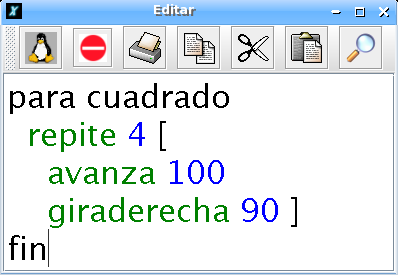
\includegraphics[scale=0.4]{Imagenes/04_Convenciones/EditorProc_01.png}
      \end{center}
   \item Pulsar 
\includegraphics[scale=0.3]{Imagenes/04_Convenciones/guardar.png} con el
      rat\'on, o hacer \texttt{Alt+Q}
   \item En la ventana del \textbf{Hist\'orico de Comandos},
      \index{Hist\'orico de Comandos} debe aparecer el mensaje:

      \textcolor{blue}{\texttt{Acaba de definir cuadrado}}
      El int\'erprete \textsc{XLogo} no detecta los posibles errores en este
      momento, sino cuando se utilice el procedimiento por primera vez.
   \item Desde ese momento, puede invocarse la orden \texttt{cuadrado} en la
      \textbf{L\'inea de Comandos}
\end{enumerate}
Los procedimientos tambi\'en pueden aprovechar las ventajas de los argumentos.
Para hacer esto, se usan \textit{variables}. \index{Variables} Una
variable es una palabra (un nombre) al que se le puede asignar un valor. 
\begin{quote}
   \noindent \textbf{Ejemplo}:
   \begin{center}
      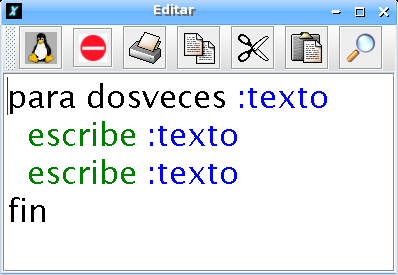
\includegraphics[scale=0.3]{Imagenes/04_Convenciones/EditorProc_02.png}
   \end{center}
   \noindent Probando el ejemplo:
   \begin{verbatim}
  dosveces [1 2 3] \end{verbatim}
   devuelve 
   \begin{verbatim}
  1 2 3
  1 2 3 \end{verbatim}
\end{quote}
Al final del manual se incluyen varios ejemplos de procedimientos.

\section{El caracter especial \textbackslash{}}
   \label{El-caracter-backslash}

El caracter \textbackslash{} (barra invertida o \textit{backslash})
\index{backslash} \index{Barra invertida} permite que las ``palabras''
(secci\'on \ref{Comandos}) contengan espacios \index{Espacios} o
saltos de l\'inea. \index{Saltos de l\'inea}
\begin{itemize}
   \item \verb+\n+ produce un salto de l\'inea
      \index{\textbackslash{}n@\texttt{\textbackslash{}n}}
   \item \verb*+\ + produce un espacio entre palabras
      \index{\verb*+\ +} (\verb*+ + representa un espacio en blanco)
\end{itemize}
\begin{quote}
   \noindent \textbf{Ejemplos}: 

   \begin{tabular}{lcccl}
      \verb+es "xlogo\ xlogo+ & & produce & &
               \texttt{xlogo xlogo} \\
      \verb+es "xlogo\nxlogo+ & & produce & &
         \texttt{xlogo} \\
         & & & & \texttt{xlogo}
   \end{tabular}
\end{quote}
Esto tiene implicaciones a la hora de obtener el caracter \textbackslash{}
en la \textbf{L\'inea de Comandos}: se debe teclear
\verb+\\+.
\index{\textbackslash{}\textbackslash{}@\texttt{\textbackslash{}\textbackslash{}}}
Todo caracter \textbackslash{} es ignorado. Este aviso es importante
en particular para la gesti\'on de archivos 
(secci\'on \ref{Manejo-de-Archivos}). Para establecer como directorio
de trabajo \verb+c:\Mis Documentos+ se debe escribir:
\begin{verbatim}
   pondirectorio "c:\\Mis\ Documentos \end{verbatim}
Nota el uso de \verb*+\ + para indicar el espacio entre
\texttt{Mis} y \texttt{Documentos}. Si se omite el doble
\textit{backslash}, la ruta definida ser\'ia interpretada como:
\begin{verbatim}
   c:Mis Documentos \end{verbatim}
y el int\'erprete mostrar\'a un mensaje de error. 

\section{May\'usculas y min\'usculas}
   \label{Mayusculas-y-minusculas}
   \index{May\'usculas y min\'usculas}

\textsc{XLogo} no distingue entre may\'usculas y min\'usculas en el caso de
nombres de procedimientos y primitivas. As\'i, en el procedimiento
\texttt{cuadrado} como fue definido antes, si escribes \texttt{CUADRADO} o
\texttt{cuAdRAdO}, el int\'erprete de comandos interpretar\'a y ejecutar\'a
correctamente \texttt{cuadrado}. Por otro lado, \textsc{XLogo} s\'i respeta
may\'usculas y min\'usculas en listas y palabras: 
\begin{verbatim}
   escribe "Hola \end{verbatim}
proporciona
\begin{verbatim}
   Hola \end{verbatim}
(la H inicial se mantuvo)

\section{Operadores y sintaxis}
   \label{Operadores-Sintaxis}
   \index{Sintaxis}

Hay dos maneras para escribir ciertos comandos. Por ejemplo, para
sumar 4 y 7, puedes usar la primitiva \texttt{suma} que espera dos
argumentos: 
\begin{verbatim}
   suma 4 7 \end{verbatim}
o puedes usar el operador \texttt{+}: 
\begin{verbatim}
   4 + 7 \end{verbatim}
Ambos tienen el mismo efecto. Esta tabla muestra la relaci\'on entre
operadores y primitivas:

\subsection{Operadores aritm\'eticos}
   \index{Operadores aritm\'eticos}

\begin{center} \begin{tabular}{|*{4}{c|}} \hline 
   \texttt{suma} \index{suma@\texttt{suma}} & 
      \texttt{diferencia} \index{diferencia@\texttt{diferencia}} &
         \texttt{producto} \index{producto@\texttt{producto}} &
            \texttt{divisi\'on} \index{divisi\'on@\texttt{divisi\'on}} \\ \hline
   \texttt{+} & \texttt{--} & * & \texttt{/} \\ \hline
\end{tabular} \end{center}

\subsection{Operadores l\'ogicos}
   \index{Operadores l\'ogicos}

\begin{center} \begin{tabular}{|*{3}{c|}} \hline 
   \texttt{o} \index{o@\texttt{o}} &
      \texttt{y} \index{y@\texttt{y}} &
         \texttt{iguales?} \index{iguales?@\texttt{iguales?}} \\ \hline
   \texttt{|}& \texttt{\&}& \texttt{=} \\ \hline
\end{tabular}\end{center}

\noindent Para comparaciones num\'ericas, disponemos de cuatro operadores sin
primitiva asociada:
\begin{itemize}
   \item El operador ``menor'': \texttt{<}\index{<@\texttt{<}}
   \item El operador ``mayor'': \texttt{>}\index{>@\texttt{>}}
\end{itemize}
Por analog\'ia con otros lenguajes, \textsc{XLogo} incorpora otros dos:
\begin{itemize}
   \item El operador ``menor o igual'': \texttt{<=}\index{<=@\texttt{<=}}
   \item El operador ``mayor o igual'': \texttt{>=}\index{>=@\texttt{>=}}
\end{itemize}
si bien es evidente que no ser\'ian estrictamente necesarios:
\begin{itemize}
   \item \texttt{a <= b} es equivalente a \texttt{no (a > b)} 
   \item \texttt{a >= b} puede sustituirse por \texttt{no (a < b)}
\end{itemize}

\textbf{Nota aclarativa}: Los operadores \texttt{|} y \texttt{\&} son
espec\'ificos de \textsc{XLogo}.\index{\&@\texttt{\&}}\index{=@\texttt{=}}
No se encuentran en otras versiones tradicionales de \textsc{Logo}.
veamos algunos ejemplos de su uso:
\begin{quote} \begin{tabular}{lccccl}
   \texttt{escribe 3+4 = 7-1}      & & devuelve & & \texttt{falso} \\
   \texttt{escribe 3=4 | 7<=49/7}  & & devuelve & & \texttt{cierto} \\
   \texttt{escribe 3=4 \& 7=49/7}  & & devuelve & & \texttt{falso}
\end{tabular} \end{quote}

\section{Las tildes}
\index{Acentuaci\'on y tildes}

Desde la versi\'on 0.9.92 las primitivas en espa\~nol \textsc{XLogo} admiten
tildes. Trat\'andose de un software para uso educativo, es importante que la
ortograf\'ia sea la adecuada.\\

\noindent Para la acentuaci\'on de las primitivas se siguen las normas
ortogr\'aficas habituales, especialmente en aquellas primitivas compuestas
por varias palabras. Por ejemplo:
\begin{itemize}
   \item \texttt{poncolorl\'apiz}. La palabra \texttt{l\'apiz} lleva tilde
      y la mantiene al formar parte de la primitiva, ya que la acentuaci\'on
      de esta recae sobre la ``\texttt{a}'' 
   \item \texttt{leelineaflujo}. Aunque \texttt{l\'inea} lleva tilde al ser
      esdr\'ujula, al pronunciar la primitiva completa, observamos que es
      una palabra llana (el acento se encuentra en la ``\texttt{u}'' de
      \texttt{flujo}), as\'i que no se le asigna tilde.

      S\'i que lleva tilde en \texttt{definel\'inea} y \texttt{finl\'inea},
      por el mismo motivo explicado antes para \texttt{l\'apiz}
   \item Se procede del mismo modo en las formas cortas de las primitivas.
      Las formas cortas de \texttt{definepol\'igono} y \texttt{finpol\'igono}
      son, respectivamente, \texttt{defpoli} y \texttt{finpoli}.
      Escuchando a los alumnos pronunciarlas, se opt\'o por considerarlas
      llanas y sin tilde.
\end{itemize}

Dicho lo anterior, debemos tener una idea sobre la distinta codificaci\'on
de caracteres que usan los Sistemas Operativos. \\

La codificaci\'on de caracteres es el m\'etodo que convierte un car\'acter de
un lenguaje natural en un c\'odigo num\'erico. Es muy habitual (m\'as de lo
que ser\'ia deseable) que los sistemas operativos (Windows, Linux, MacOS,
Solaris, \ldots) usen distintos sistemas de codificaci\'on. Existen varias
normas: ASCII, Unicode, UTF, ISO, \ldots, y eso afecta negativamente a los
caracteres especiales del espa\~nol:
\begin{itemize}
   \item Vocales acentuadas: \'a, \'e, \'i, \'o, \'u
   \item Letras e\~ne y ``cedilla'': \~n y \c{c}
   \item Apertura de exclamaci\'on, interrogaci\'on, \ldots: ?`, !` , \ldots.
\end{itemize}

Si tienes intenci\'on de compartir tus programas por Internet, intenta evitar
estos caracteres y utiliza primitivas sin tilde. Si est\'as en una aula,
recomendamos el uso acentuado de las mismas.